
\documentclass[11pt,a4paper]{article}
\usepackage[margin=2.2cm]{geometry}
\usepackage[utf8]{inputenc}
\usepackage[T1]{fontenc}
\usepackage{amsmath,amssymb,mathtools,bm}
\usepackage{graphicx,booktabs,longtable,array,microtype,xcolor,hyperref,fancyhdr,enumitem}
\graphicspath{{../images/}}
\definecolor{navy}{HTML}{17324D}\definecolor{rust}{HTML}{A33A2B}\definecolor{green}{HTML}{176B4D}
\hypersetup{colorlinks=true,linkcolor=navy,urlcolor=rust,citecolor=green}
\pagestyle{fancy}\fancyhf{}\lhead{Auditoria estrutural da RH}\rhead{Dossiê técnico}\cfoot{\thepage}
\newcommand{\Drad}{\mathfrak D_{\mathrm{rad}}}
\newcommand{\Dpar}{\Delta_{\mathrm{par}}}
\newcommand{\status}[2]{\par\noindent\colorbox{#1!12}{\textcolor{#1}{\textbf{#2}}}\quad}
\begin{document}

\begin{titlepage}\centering{\Huge\sffamily\bfseries Atlas completo de visualizações\par}\vfill{\Large Auditoria estrutural e formalização lógica\par}\vfill Agosto de 2026\end{titlepage}
\tableofcontents\clearpage
\section{Detector geométrico}
\begin{center}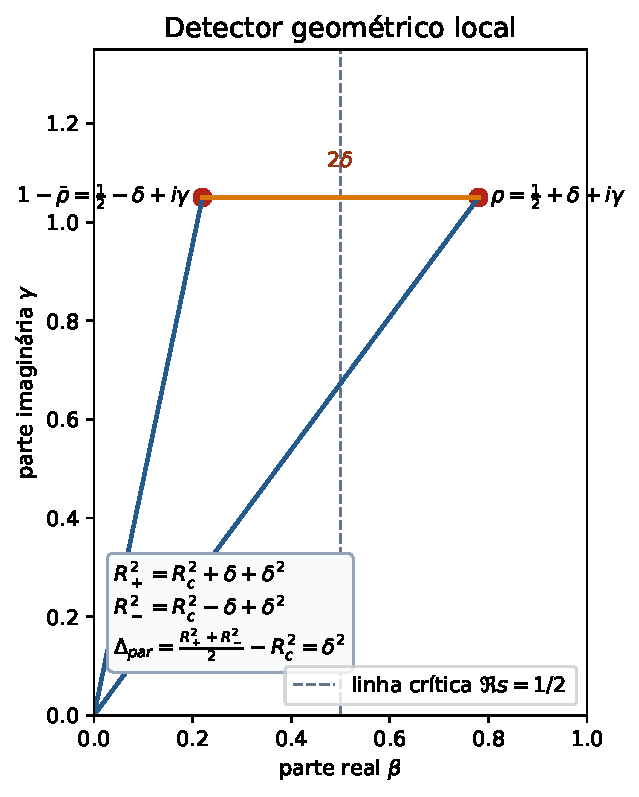
\includegraphics[width=.98\linewidth,height=.78\textheight,keepaspectratio]{01-detector-geometrico.pdf}\end{center}\clearpage
\section{Quarteto e simetrias}
\begin{center}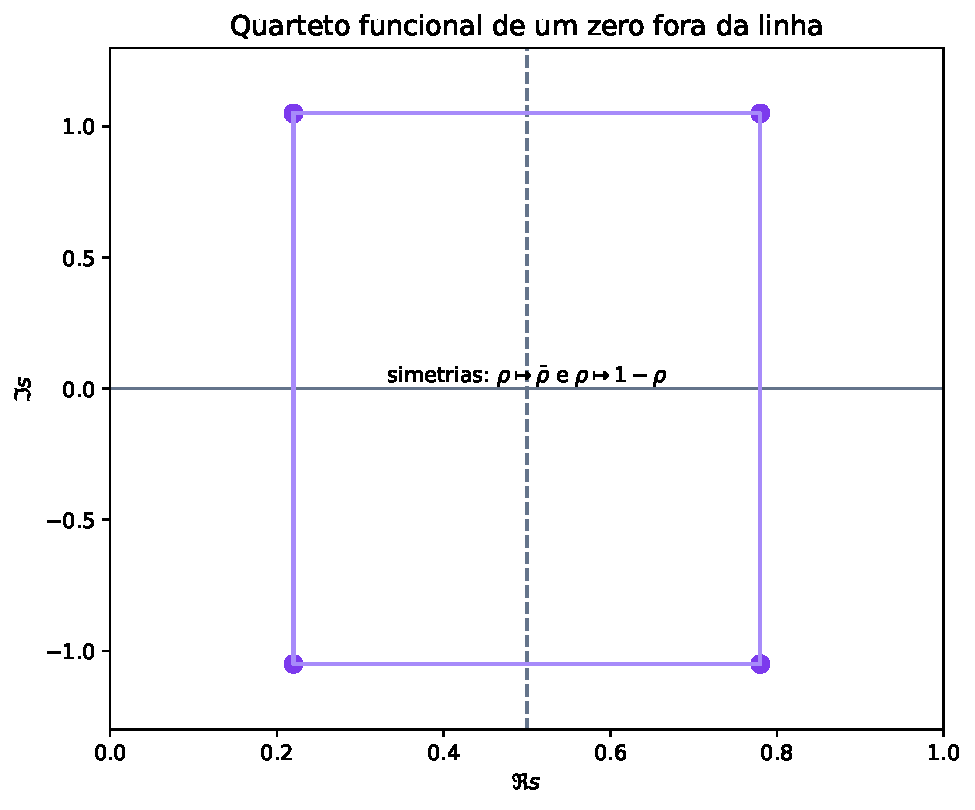
\includegraphics[width=.98\linewidth,height=.78\textheight,keepaspectratio]{02-quarteto-simetrias.pdf}\end{center}\clearpage
\section{Parábola do defeito local}
\begin{center}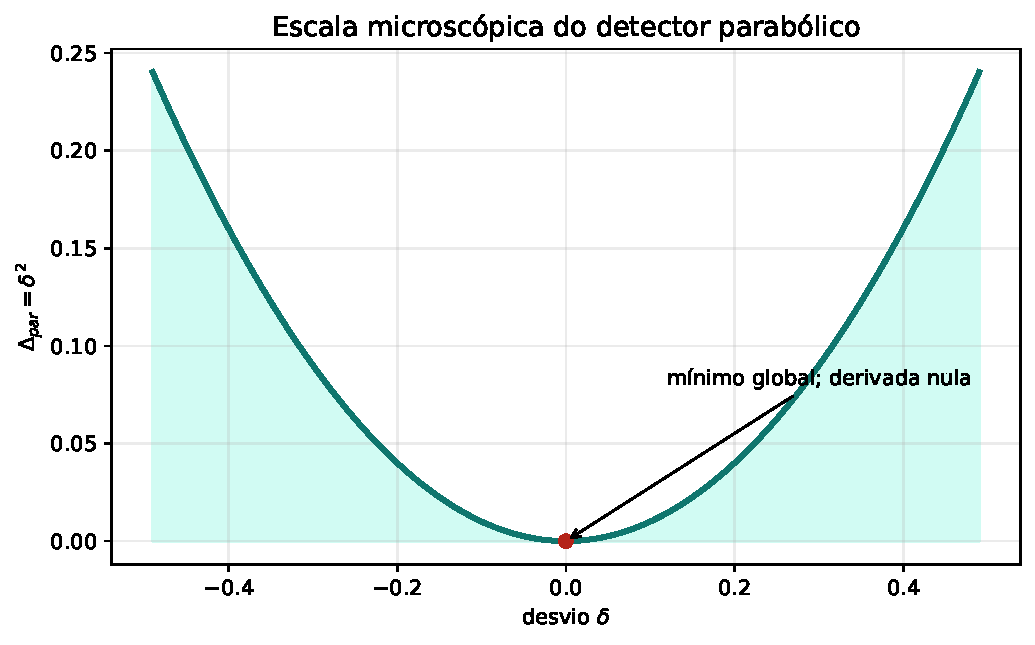
\includegraphics[width=.98\linewidth,height=.78\textheight,keepaspectratio]{03-parabola-delta.pdf}\end{center}\clearpage
\section{Peso versus desvio}
\begin{center}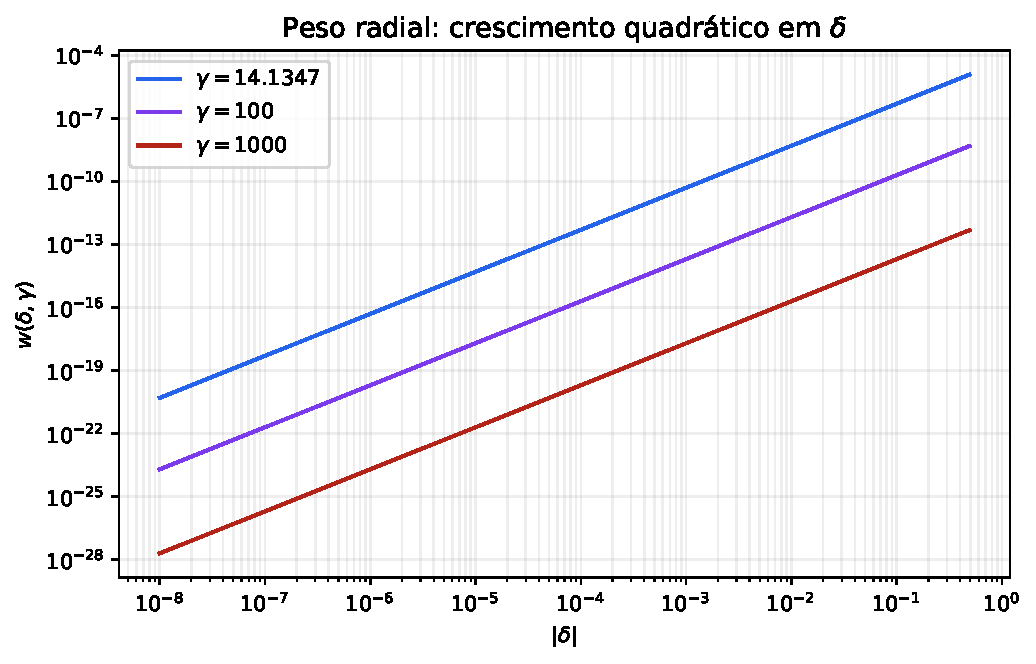
\includegraphics[width=.98\linewidth,height=.78\textheight,keepaspectratio]{04-peso-versus-delta.pdf}\end{center}\clearpage
\section{Decaimento com a altura}
\begin{center}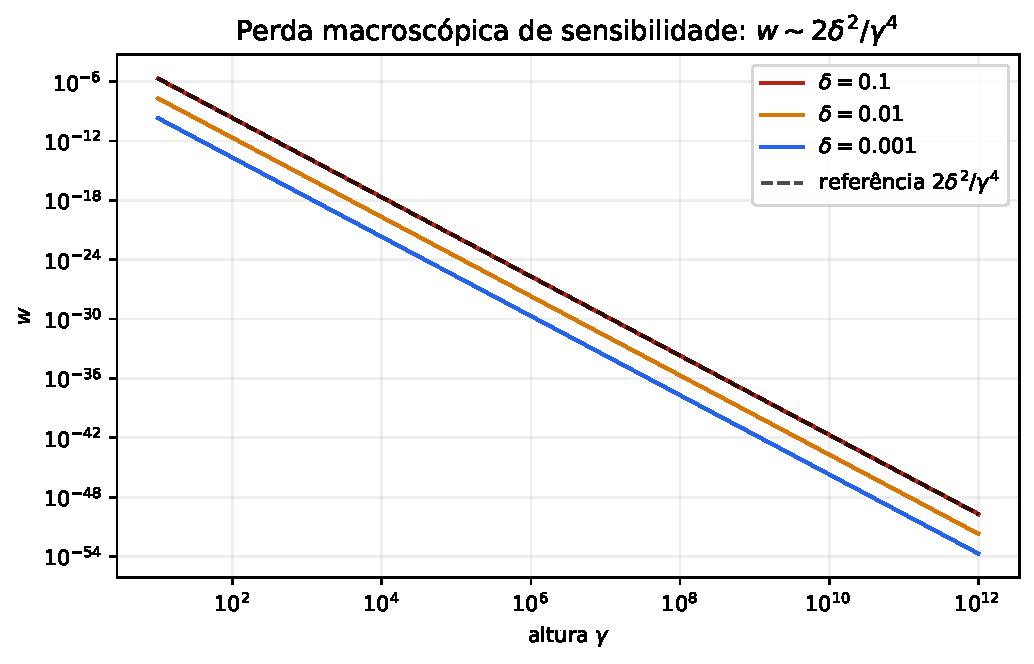
\includegraphics[width=.98\linewidth,height=.78\textheight,keepaspectratio]{05-decaimento-gamma.pdf}\end{center}\clearpage
\section{Mapa multiescala}
\begin{center}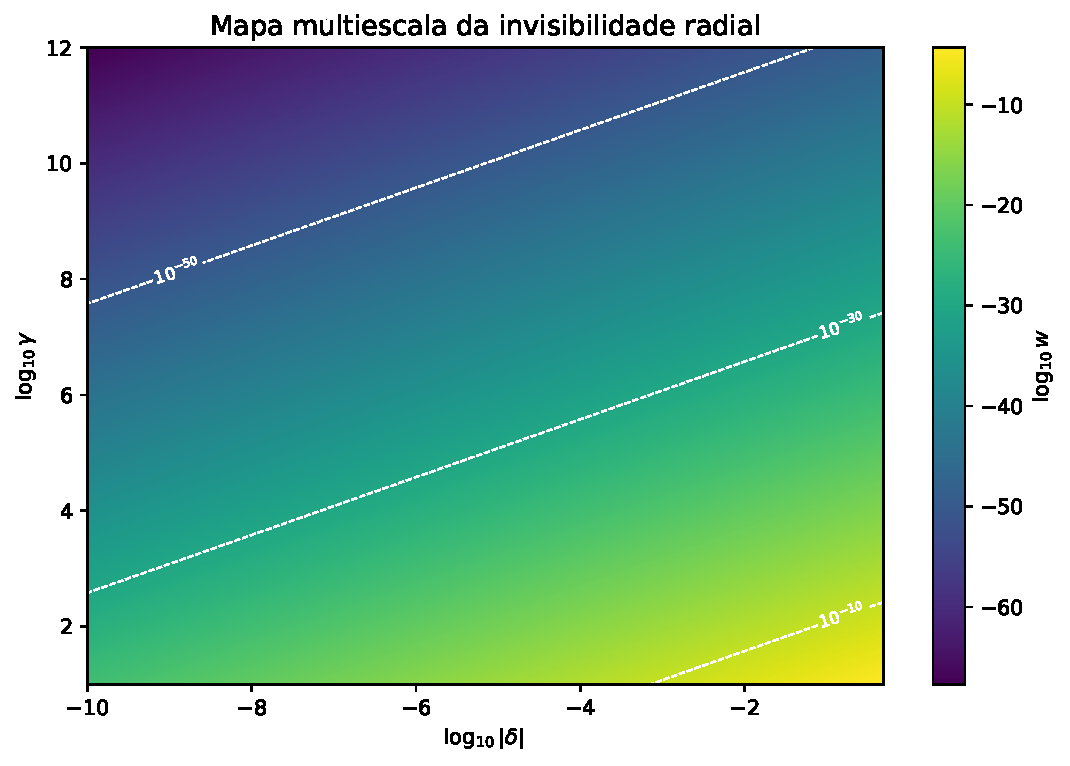
\includegraphics[width=.98\linewidth,height=.78\textheight,keepaspectratio]{06-mapa-log-peso.pdf}\end{center}\clearpage
\section{Condicionamento numérico}
\begin{center}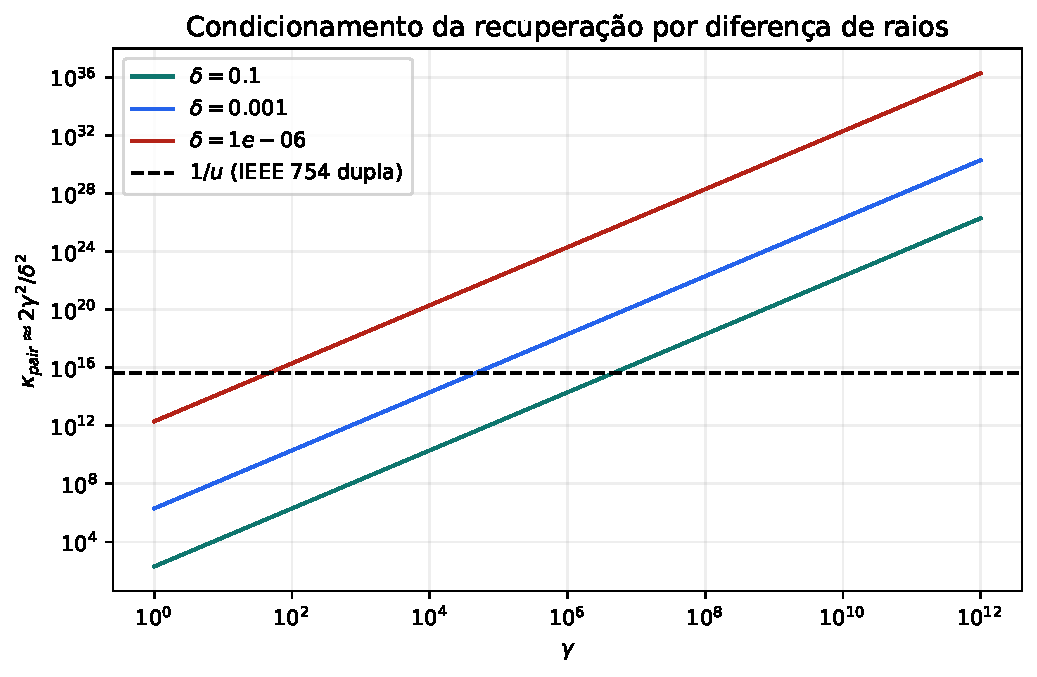
\includegraphics[width=.98\linewidth,height=.78\textheight,keepaspectratio]{07-condicionamento.pdf}\end{center}\clearpage
\section{Hierarquia do defeito}
\begin{center}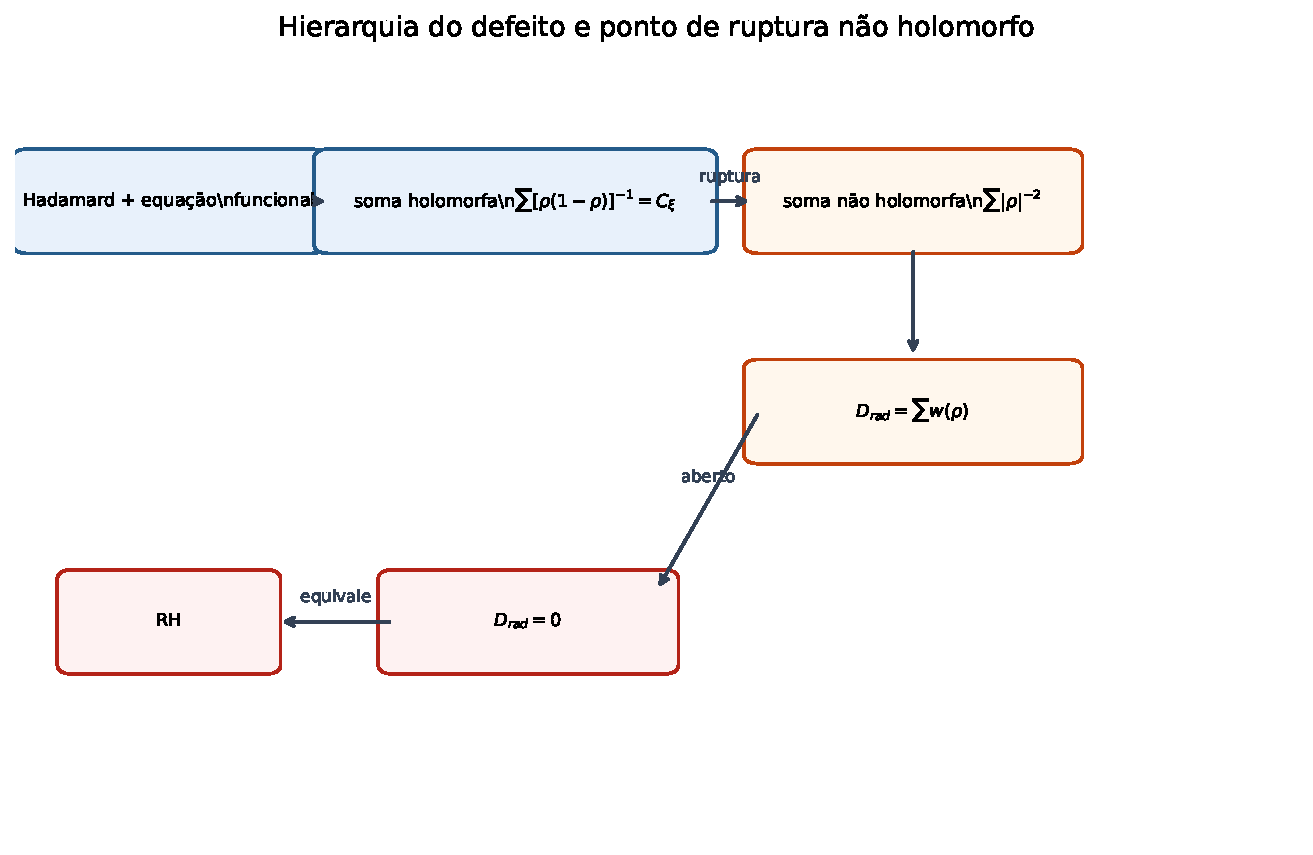
\includegraphics[width=.98\linewidth,height=.78\textheight,keepaspectratio]{08-hierarquia-defeito.pdf}\end{center}\clearpage
\section{Classificação lógica}
\begin{center}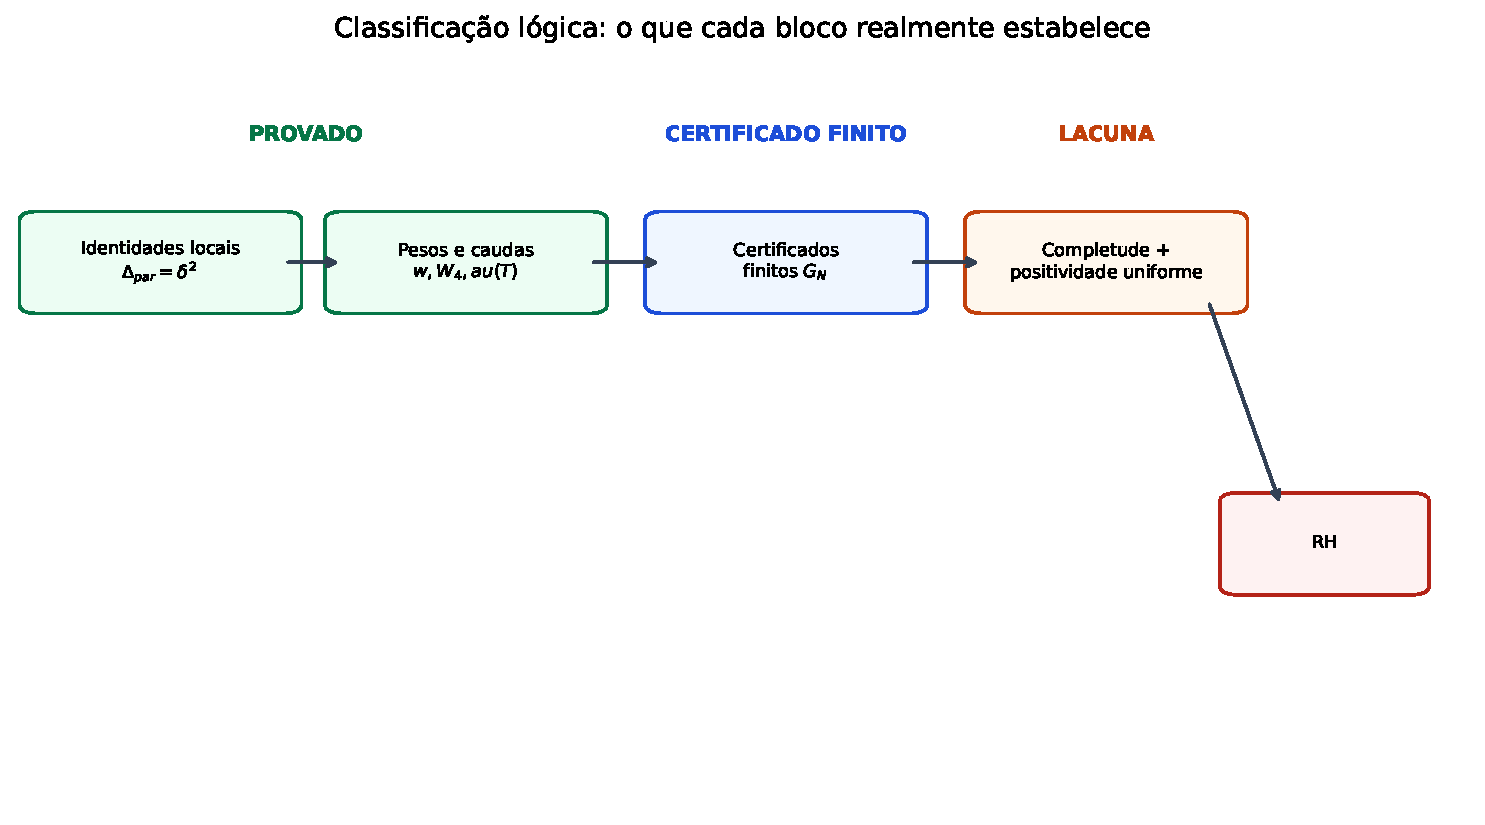
\includegraphics[width=.98\linewidth,height=.78\textheight,keepaspectratio]{09-status-logico.pdf}\end{center}\clearpage
\section{Três vias de fechamento}
\begin{center}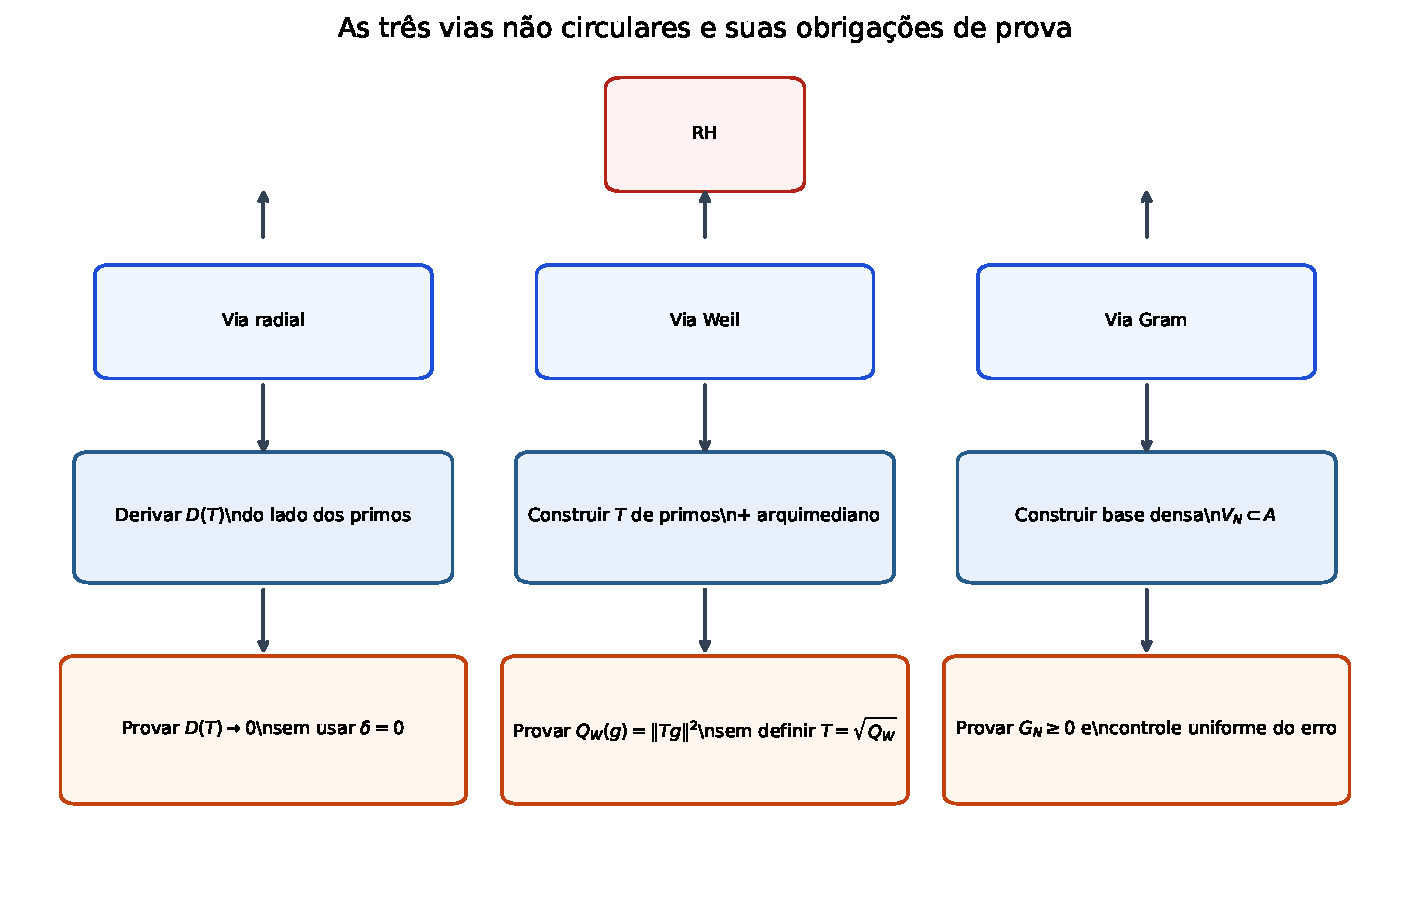
\includegraphics[width=.98\linewidth,height=.78\textheight,keepaspectratio]{10-tres-vias.pdf}\end{center}\clearpage
\section{Teste de circularidade}
\begin{center}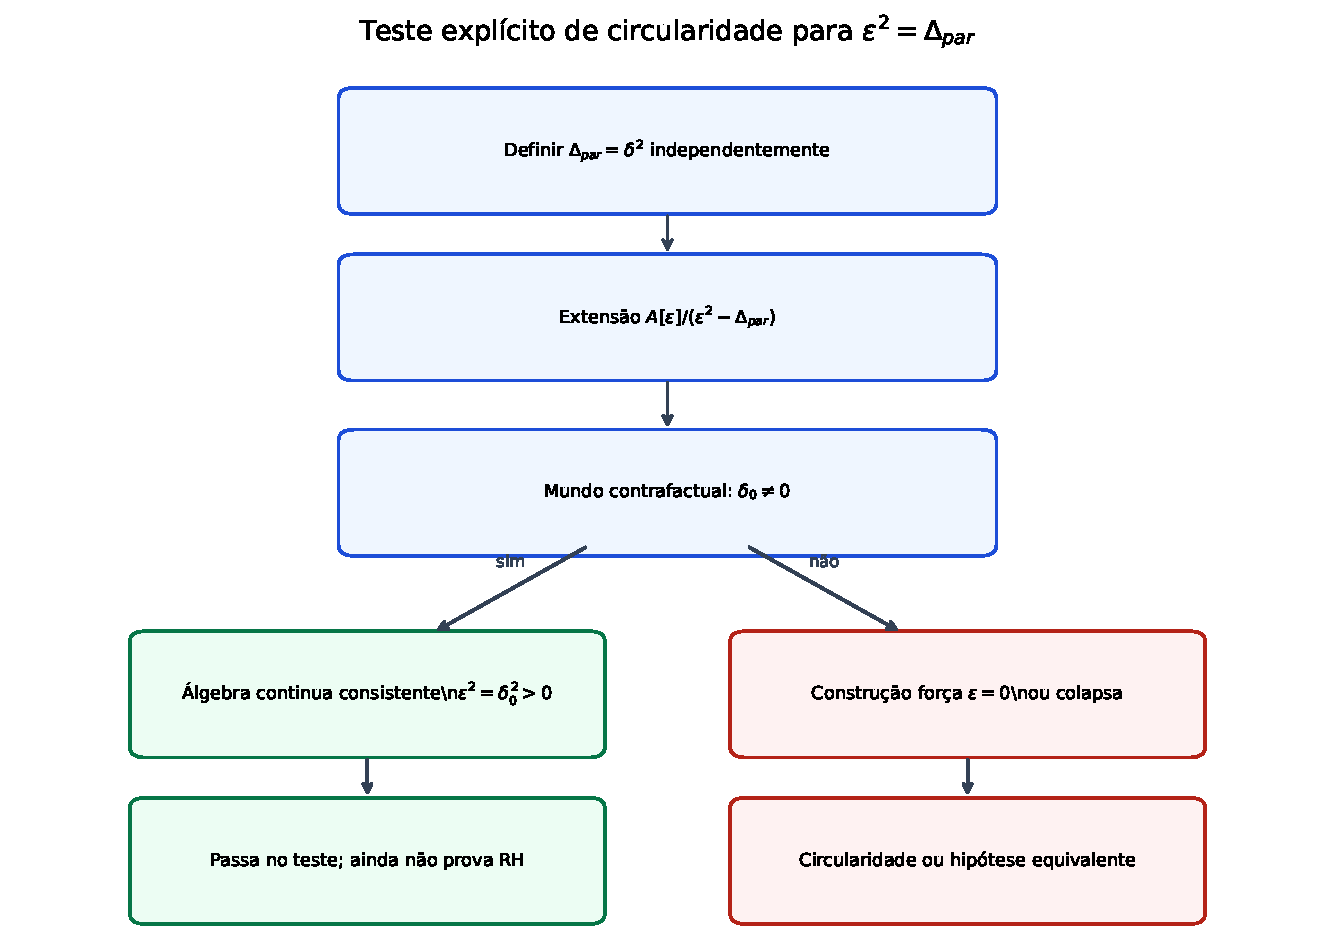
\includegraphics[width=.98\linewidth,height=.78\textheight,keepaspectratio]{11-teste-circularidade.pdf}\end{center}\clearpage
\section{Matriz hermitiana de dimensão 13}
\begin{center}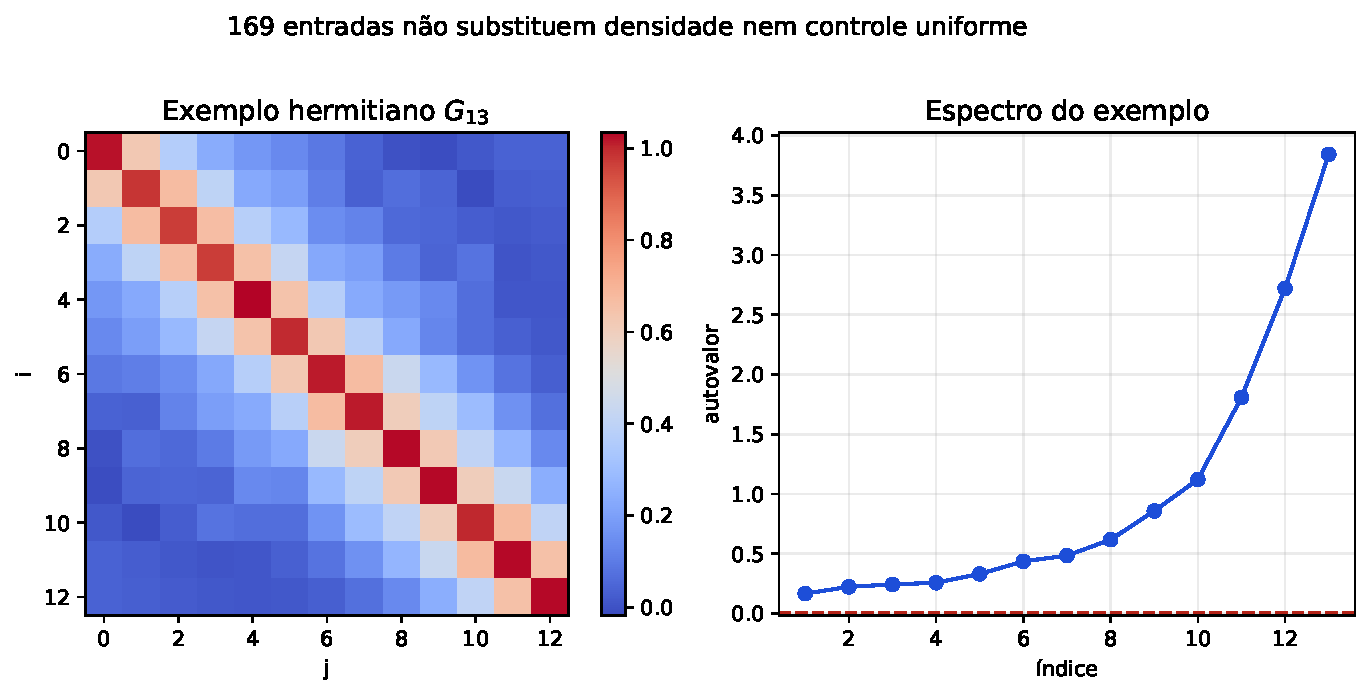
\includegraphics[width=.98\linewidth,height=.78\textheight,keepaspectratio]{12-matriz-g13.pdf}\end{center}\clearpage
\end{document}
